\def\x{{\mathbf x}}
\def\f{{\mathbf f}}

\def\S{{\cal S}}
\def\T{{\cal T}}

\def\R{{\mathds R}}

\def\tf{{\theta_f}}
\def\td{{\theta_d}}
\def\ty{{\theta_y}}
\def\htf{{\hat\theta_f}}
\def\htd{{\hat\theta_d}}
\def\hty{{\hat\theta_y}}


\section{An alternative optimization approach}
\label{sect:appendix_alternative}

There exists an alternative construction (inspired by \cite{Goodfellow14}) that leads to the same updates \eq{upd1}-\eq{upd3}. Rather than using the gradient reversal layer, the construction introduces two different loss functions for the domain classifier. Minimization of the first domain loss ($ L_{d+} $) should lead to a better domain discrimination, while the second domain loss ($ L_{d-} $) is minimized when the domains are distinct. Stochastic updates for $ \theta_f $ and $ \theta_d $ are then defined as:
\begin{align*}
  \tf \quad &\longleftarrow \quad \tf \;-\; \mu \left(\frac{\partial L^i_y}{\partial \tf} + \frac{\partial L^i_{d-}}{\partial \tf} \right)\\
  \td \quad &\longleftarrow \qquad \td \;-\; \mu \frac{\partial L^i_{d+}}{\partial \td} \, ,
\end{align*}
Thus, different parameters participate in the optimization of different losses

In this framework, the gradient reversal layer constitutes a special case, corresponding  to the pair of domain losses $ (L_d, -\lambda L_d) $. However, other pairs of loss functions can be used. One example would be the binomial cross-entropy \cite{Goodfellow14}:
\begin{equation*}
  L_{d+}(q, d) = \sum_{i = 1..N} d_i \log(q_i) + (1 - d_i) \log(1 - q_i) \, ,
\end{equation*}
where $ d $ indicates domain indices and $ q $ is an output of the predictor. In that case ``adversarial'' loss is easily obtained by swapping domain labels, i.e.\ $ L_{d-}(q, d) = L_{d+}(q, 1 - d) $. This particular pair has a potential advantage of producing stronger gradients at early learning stages if the domains are quite dissimilar. In our experiments, however, we did not observe any significant improvement resulting from this choice of losses.

\section{CNN architectures}
\label{sect:appendix_archs}

\begin{figure*}[t]
  \definecolor{fnodebottom}{RGB}{132,170,81}
  \definecolor{fnodetop}{RGB}{172,222,106}
  \definecolor{cnodebottom}{RGB}{120,128,164}
  \definecolor{cnodetop}{RGB}{158,167,218}
  \definecolor{dnodebottom}{RGB}{174,109,146}
  \definecolor{dnodetop}{RGB}{230,141,192}
  \centering
  \subfigure[MNIST architecture]{%
    \scalebox{0.65}{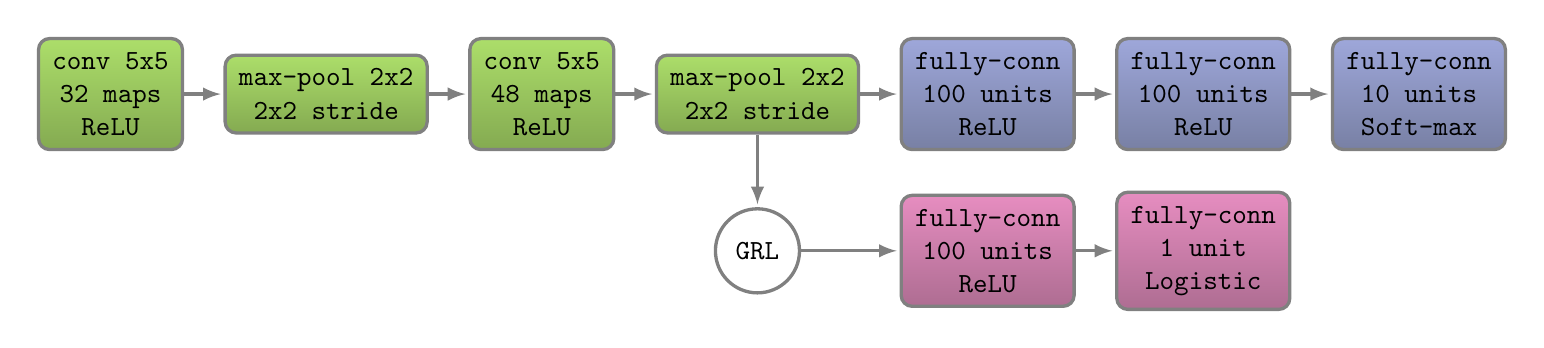
\begin{tikzpicture}[
  black!50, text=black,
  node distance=4mm,
  grlnode/.style={
    align=center,
    circle,minimum size=6mm,
    inner sep=5pt,
    very thick,draw=black!50,
    font=\ttfamily
  },
  fnode/.style={
    align=center,
    % The shape:
    rectangle,minimum size=6mm,rounded corners,
    % The rest
    inner sep=5pt,
    very thick,draw=black!50,
    top color=fnodetop,bottom color=fnodebottom,
    font=\ttfamily},
  cnode/.style={
    fnode,top color=cnodetop,bottom color=cnodebottom},
  dnode/.style={
    fnode,top color=dnodetop,bottom color=dnodebottom},
  vhedge/.style={
    rounded corners,to path=|- (\tikztotarget)}]
  \matrix[row sep=5mm,column sep=5mm] {
    \node (conv1) [fnode] {conv 5x5\\32 maps\\ReLU}; &
    \node (pool1) [fnode] {max-pool 2x2\\2x2 stride}; &
    \node (conv2) [fnode] {conv 5x5\\48 maps\\ReLU}; &
    \node (pool2) [fnode] {max-pool 2x2\\2x2 stride}; &
  
    \node (fc3)   [cnode] {fully-conn\\100 units\\ReLU}; &
    \node (fc4)   [cnode] {fully-conn\\100 units\\ReLU}; &
    \node (fc5)   [cnode] {fully-conn\\10 units\\Soft-max}; \\
  
    & & &
    \node (grl) [grlnode] {GRL}; &
  
    \node (fc1_d) [dnode] {fully-conn\\100 units\\ReLU}; &
    \node (fc2_d) [dnode] {fully-conn\\1 unit\\Logistic}; \\
  };
  
  \path (conv1) edge[-latex,shorten >=1pt,very thick] (pool1);
  \path (pool1) edge[-latex,shorten >=1pt,very thick] (conv2);
  \path (conv2) edge[-latex,shorten >=1pt,very thick] (pool2);
  \path (pool2) edge[-latex,shorten >=1pt,very thick] (fc3);
  \path (fc3)   edge[-latex,shorten >=1pt,very thick] (fc4);
  \path (fc4)   edge[-latex,shorten >=1pt,very thick] (fc5);
  
  \path (pool2.south) edge[-latex,shorten >=1pt,very thick] (grl.north);
  \path (grl) edge[-latex,shorten >=1pt,very thick] (fc1_d);
  \path (fc1_d) edge[-latex,shorten >=1pt,very thick] (fc2_d);
\end{tikzpicture}
}}\\
  \subfigure[SVHN architecture]{%
    \scalebox{0.65}{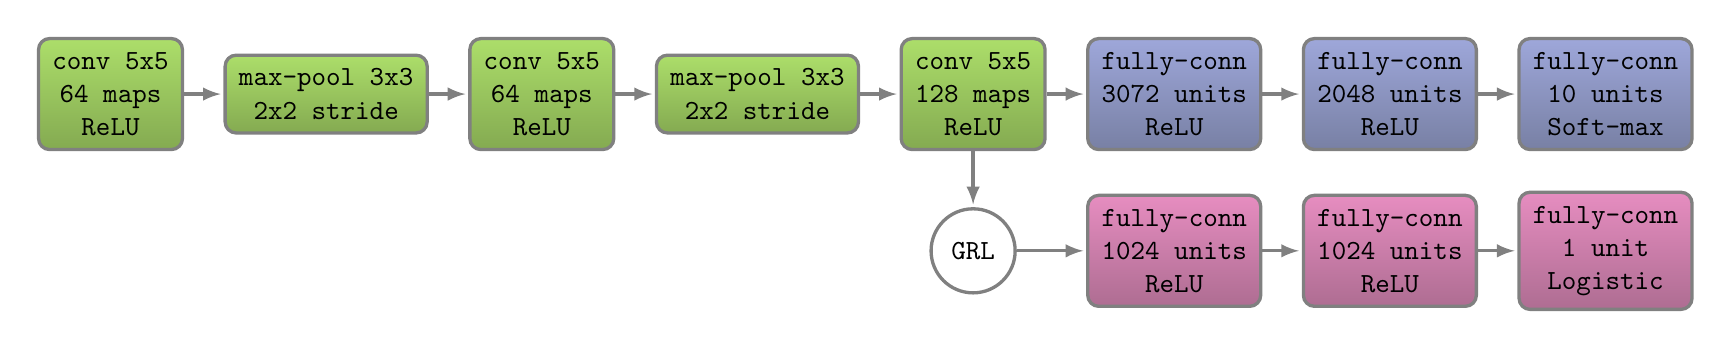
\begin{tikzpicture}[
  black!50, text=black,
  node distance=4mm,
  grlnode/.style={
    align=center,
    circle,minimum size=6mm,
    inner sep=5pt,
    very thick,draw=black!50,
    font=\ttfamily
  },
  fnode/.style={
    align=center,
    % The shape:
    rectangle,minimum size=6mm,rounded corners,
    % The rest
    inner sep=5pt,
    very thick,draw=black!50,
    top color=fnodetop,bottom color=fnodebottom,
    font=\ttfamily},
  cnode/.style={
    fnode,top color=cnodetop,bottom color=cnodebottom},
  dnode/.style={
    fnode,top color=dnodetop,bottom color=dnodebottom},
  vhedge/.style={
    rounded corners,to path=|- (\tikztotarget)}]
  \matrix[row sep=5mm,column sep=5mm] {
    \node (conv1) [fnode] {conv 5x5\\64 maps\\ReLU}; &
    \node (pool1) [fnode] {max-pool 3x3\\2x2 stride}; &
    \node (conv2) [fnode] {conv 5x5\\64 maps\\ReLU}; &
    \node (pool2) [fnode] {max-pool 3x3\\2x2 stride}; &
    \node (conv3) [fnode] {conv 5x5\\128 maps\\ReLU}; &
  
    \node (fc4)   [cnode] {fully-conn\\3072 units\\ReLU}; &
    \node (fc5)   [cnode] {fully-conn\\2048 units\\ReLU}; &
    \node (fc6)   [cnode] {fully-conn\\10 units\\Soft-max}; \\
  
    & & & &
    \node (grl) [grlnode] {GRL}; &
    \node (fc1_d) [dnode] {fully-conn\\1024 units\\ReLU}; &
    \node (fc2_d) [dnode] {fully-conn\\1024 units\\ReLU}; &
    \node (fc3_d) [dnode] {fully-conn\\1 unit\\Logistic}; \\
  };
  
  \path (conv1) edge[-latex,shorten >=1pt,very thick] (pool1);
  \path (pool1) edge[-latex,shorten >=1pt,very thick] (conv2);
  \path (conv2) edge[-latex,shorten >=1pt,very thick] (pool2);
  \path (pool2) edge[-latex,shorten >=1pt,very thick] (conv3);
  \path (conv3) edge[-latex,shorten >=1pt,very thick] (fc4);
  \path (fc4)   edge[-latex,shorten >=1pt,very thick] (fc5);
  \path (fc5)   edge[-latex,shorten >=1pt,very thick] (fc6);
  
  \path (conv3.south) edge[-latex,shorten >=1pt,very thick] (grl.north);
  \path (grl) edge[-latex,shorten >=1pt,very thick] (fc1_d);
  \path (fc1_d) edge[-latex,shorten >=1pt,very thick] (fc2_d);
  \path (fc2_d) edge[-latex,shorten >=1pt,very thick] (fc3_d);
\end{tikzpicture}
}}\\
  \subfigure[GTSRB architecture]{%
    \scalebox{0.65}{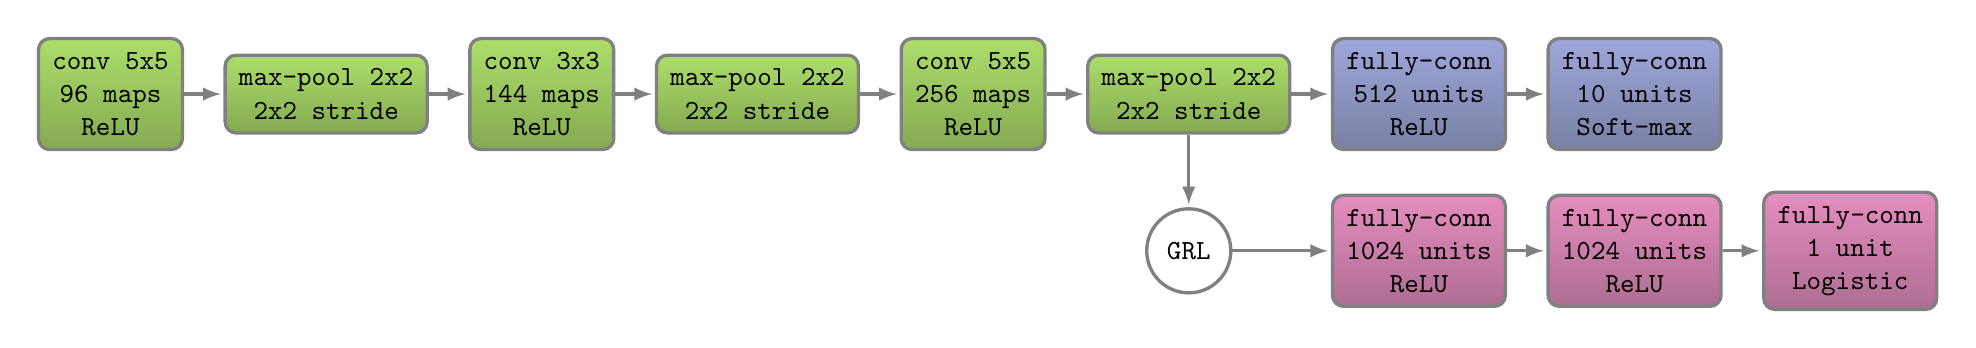
\begin{tikzpicture}[
  black!50, text=black,
  node distance=4mm,
  grlnode/.style={
    align=center,
    circle,minimum size=6mm,
    inner sep=5pt,
    very thick,draw=black!50,
    font=\ttfamily
  },
  fnode/.style={
    align=center,
    % The shape:
    rectangle,minimum size=6mm,rounded corners,
    % The rest
    inner sep=5pt,
    very thick,draw=black!50,
    top color=fnodetop,bottom color=fnodebottom,
    font=\ttfamily},
  cnode/.style={
    fnode,top color=cnodetop,bottom color=cnodebottom},
  dnode/.style={
    fnode,top color=dnodetop,bottom color=dnodebottom},
  vhedge/.style={
    rounded corners,to path=|- (\tikztotarget)}]
  \matrix[row sep=5mm,column sep=5mm] {
    \node (conv1) [fnode] {conv 5x5\\96 maps\\ReLU}; &
    \node (pool1) [fnode] {max-pool 2x2\\2x2 stride}; &
    \node (conv2) [fnode] {conv 3x3\\144 maps\\ReLU}; &
    \node (pool2) [fnode] {max-pool 2x2\\2x2 stride}; &
    \node (conv3) [fnode] {conv 5x5\\256 maps\\ReLU}; &
    \node (pool3) [fnode] {max-pool 2x2\\2x2 stride}; &
  
    \node (fc4)   [cnode] {fully-conn\\512 units\\ReLU}; &
    \node (fc5)   [cnode] {fully-conn\\10 units\\Soft-max}; \\
  
    & & & & &
    \node (grl) [grlnode] {GRL}; &
    \node (fc1_d) [dnode] {fully-conn\\1024 units\\ReLU}; &
    \node (fc2_d) [dnode] {fully-conn\\1024 units\\ReLU}; &
    \node (fc3_d) [dnode] {fully-conn\\1 unit\\Logistic}; \\
  };
  
  \path (conv1) edge[-latex,shorten >=1pt,very thick] (pool1);
  \path (pool1) edge[-latex,shorten >=1pt,very thick] (conv2);
  \path (conv2) edge[-latex,shorten >=1pt,very thick] (pool2);
  \path (pool2) edge[-latex,shorten >=1pt,very thick] (conv3);
  \path (conv3) edge[-latex,shorten >=1pt,very thick] (pool3);
  \path (pool3) edge[-latex,shorten >=1pt,very thick] (fc4);
  \path (fc4)   edge[-latex,shorten >=1pt,very thick] (fc5);
  
  \path (pool3.south) edge[-latex,shorten >=1pt,very thick] (grl.north);
  \path (grl) edge[-latex,shorten >=1pt,very thick] (fc1_d);
  \path (fc1_d) edge[-latex,shorten >=1pt,very thick] (fc2_d);
  \path (fc2_d) edge[-latex,shorten >=1pt,very thick] (fc3_d);
\end{tikzpicture}
}}\\
%   \subfigure[CIFAR-10 architecture]{%
%     \scalebox{0.65}{\input{./figures/archs/cifar10.tikz}}}
  \caption{CNN architectures used in the experiments. Boxes correspond to transformations applied to the data. Color-coding is the same as in \fig{arch}.}
  \label{fig:exper_archs}
\end{figure*}

Four different architectures were used in our experiments (first three are shown in \fig{exper_archs}):
\begin{itemize}
  \item A smaller one (a) if the source domain is MNIST. This architecture was inspired by the classical LeNet-5 \cite{LeCun98}.
  \item (b) for the experiments involving SVHN dataset. This one is adopted from \cite{Srivastava14}.
  \item (c) in the {\sc Syn Sings} $ \rightarrow $ {\sc GTSRB} setting. We used the single-CNN baseline from \cite{Cirecsan12} as our starting point.
  \item Finally, we use pre-trained \texttt{AlexNet} from the \texttt{Caffe}-package \cite{Jia14} for the {\sc Office} domains. Adaptation architecture is identical to \cite{Tzeng14}: 2-layer domain classifier ($x\rightarrow1024\rightarrow1024\rightarrow2$) is attached to the $ 256 $-dimensional bottleneck of \texttt{fc7}.  
\end{itemize}
The domain classifier branch in all cases is somewhat arbitrary (better adaptation performance might be attained if this part of the architecture is tuned).

\section{Training procedure}
\label{sect:appendix_training}

We use stochastic gradient descent with 0.9 momentum and the learning rate annealing described by the following formula:
\begin{equation*}
  \mu_p = \frac{\mu_0}{(1 + \alpha \cdot p)^\beta} \, , 
\end{equation*}
where $ p $ is the training progress linearly changing from 0 to 1, $ \mu_0 = 0.01 $, $ \alpha = 10 $ and $ \beta = 0.75 $ (the schedule was optimized to promote convergence and low error on the \emph{source} domain).

Following \cite{Srivastava14} we also use dropout and $ \ell_2 $-norm restriction when we train the SVHN architecture.

% \section{Adaptation of pretrained networks}

% We tried to apply our approach to some other common datasets used for evaluation of the domain adaptation algorithms, namely {\it Office} \cite{Saenko10} and {\it Bing-Caltech} \cite{Bergamo10}. Due to lack of time we opted for the fine-tuning of the CNN pre-trained on the ImageNet \cite{Donahue14}. Apparently this kind of regime is harder for the proposed method as we were unable to obtain any significant improvements over the results reported in \cite{Donahue14}. One possible explanation for this effect would be that the backpropagation-based adaptation with a uniform processing of both domains (we are not using separate networks for each domain) fails to sensibly change the layers up to the label predictor as those are already optimized to the convergence during the pre-training stage \cite{Erhan10}. The latter ruins the performance of our algorithm if the pre-trained model intermixes the domains poorly. Note that this problem is not as noticeable for the supervised knowledge transfer as it seems that the discrepancy between the features' distributions can be successfully hidden by retraining of the top layers. 

% \section{Additional experiments}
% The first four datasets are the well-known MNIST dataset  and its modifications. The modifications include:
% \begin{itemize}
%   \item MNIST (D): {\it Binary dilation with a $ 3 \times 3 $ all-ones structuring element.} This operation makes strokes thicker and may fill small holes thereby introducing additional challenge to the classification task.
%   \item MNIST ($ \max $, BG): {\it Blending white digits over the patches randomly extracted from photos (BSDS500).} While leaving meaningful pixels as they are, this modification adds strong background clutter. % Convolutional neural networks (except for the fully-connected layers) do not use spatial information therefore cannot simply learn to discard pixels  
%   \item MNIST ($ | \Delta | $, BG): {\it Difference-blending digits over the patches randomly extracted from photos (BSDS500).} This operation is formally defined for two images $ I^{1}, I^{2} $ as $ I_{ijk}^{out} = | I_{ijk}^{1} - I_{ijk}^{2} | $, where $ i, j $ are the coordinates of a pixel and $ k $ is a channel index. In other words, an output sample is produced by taking a patch from a photo and inverting its pixels at positions corresponding to the pixels of a digit. For a human the classification task becomes only slightly harder compared to the original dataset (the digits are still clearly distinguishable) whereas for a CNN trained on MNIST this domain is quite distinct: the background and the strokes are no longer constant.   
% \end{itemize}

% In the first three experiments, we deal with the MNIST dataset: a classifier is trained on the original dataset while being adapted to perform well on a particular modification of the source domain. The three target domains can be ordered in terms of the similarity to the source domain (which can be judged based on the performance of the classifier trained on the source domain and applied to the target domain). As expected, domain adaptation is easiest for the target domain that is closest to the source ({\sc MNIST (d)}), and our method is able to cover three quarters of the performance gap between the source-trained and target-trained classifiers (i.e. lower and upper bounds). 
